\subsection{Code Clones}
\begin{frame}{\insertsubsection}
	\leftorright{
		\todots
	}{
		\todots
	}
\end{frame}
% cloning in single-system engineering, levels of clones?
% cloning in the large, considered harmful
% clone-and-own: even more problematic

\subsection{Feature Traceability}
\begin{frame}{\insertsubsection}
	\leftandright{
		\mydefinition{Feature Traceability \mysource{\fospl\mypage{54}}}{\mycite{Feature traceability is the ability to trace a feature from the problem space (for example, the feature model) to the solution space (that is, its manifestation in design and code artifacts).}}
		\todo{all terms introduced?}
	}{
		\myexampletight{Feature Traceability with Colored Source Code}{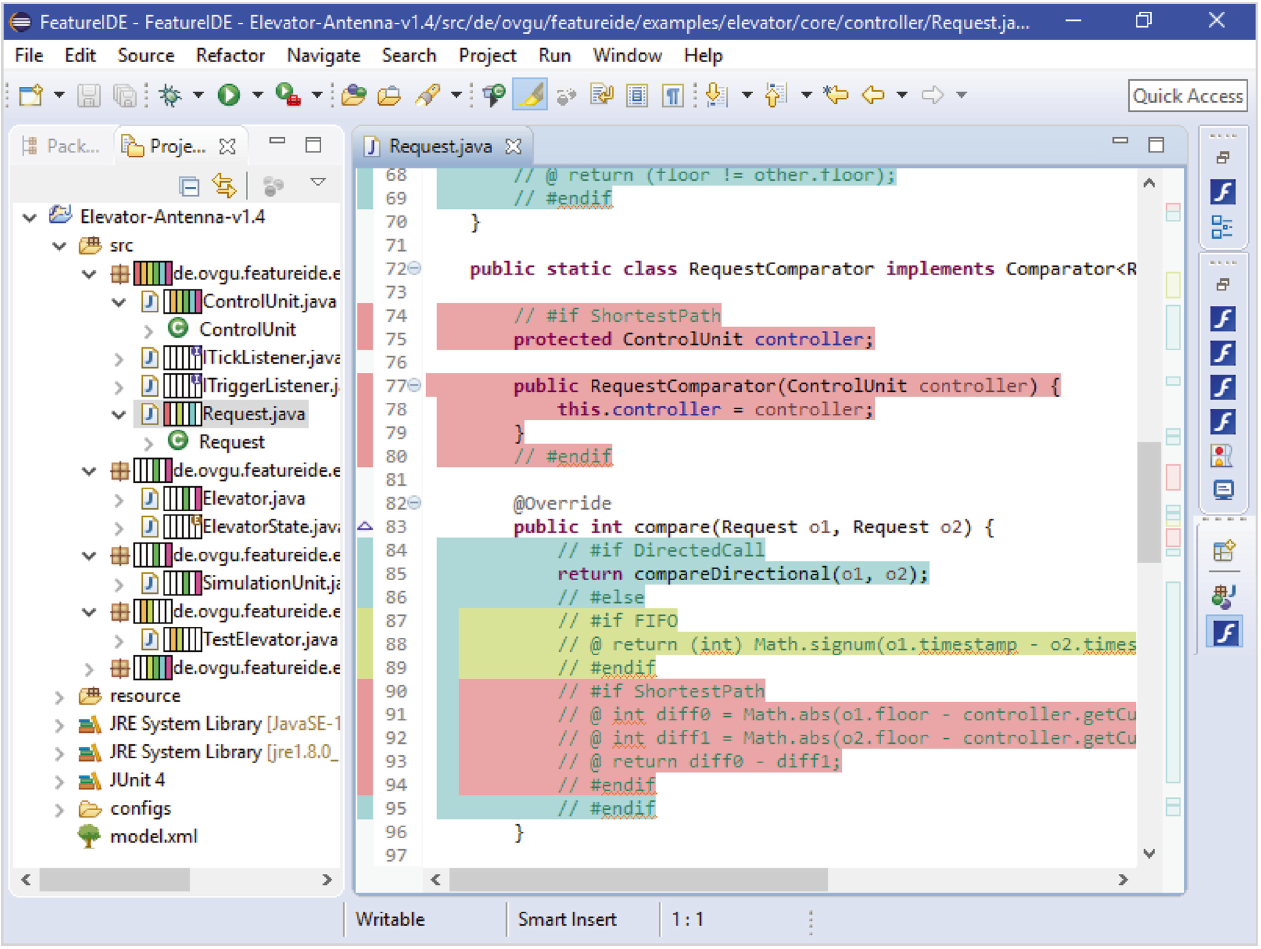
\includegraphics[width=\linewidth]{feature-traceability}}
	}
\end{frame}

\subsection{Automated Generation}
\begin{frame}{\insertsubsection}
	\leftorright{
		\todots
	}{
		\href{https://pxhere.com/en/photo/920906}{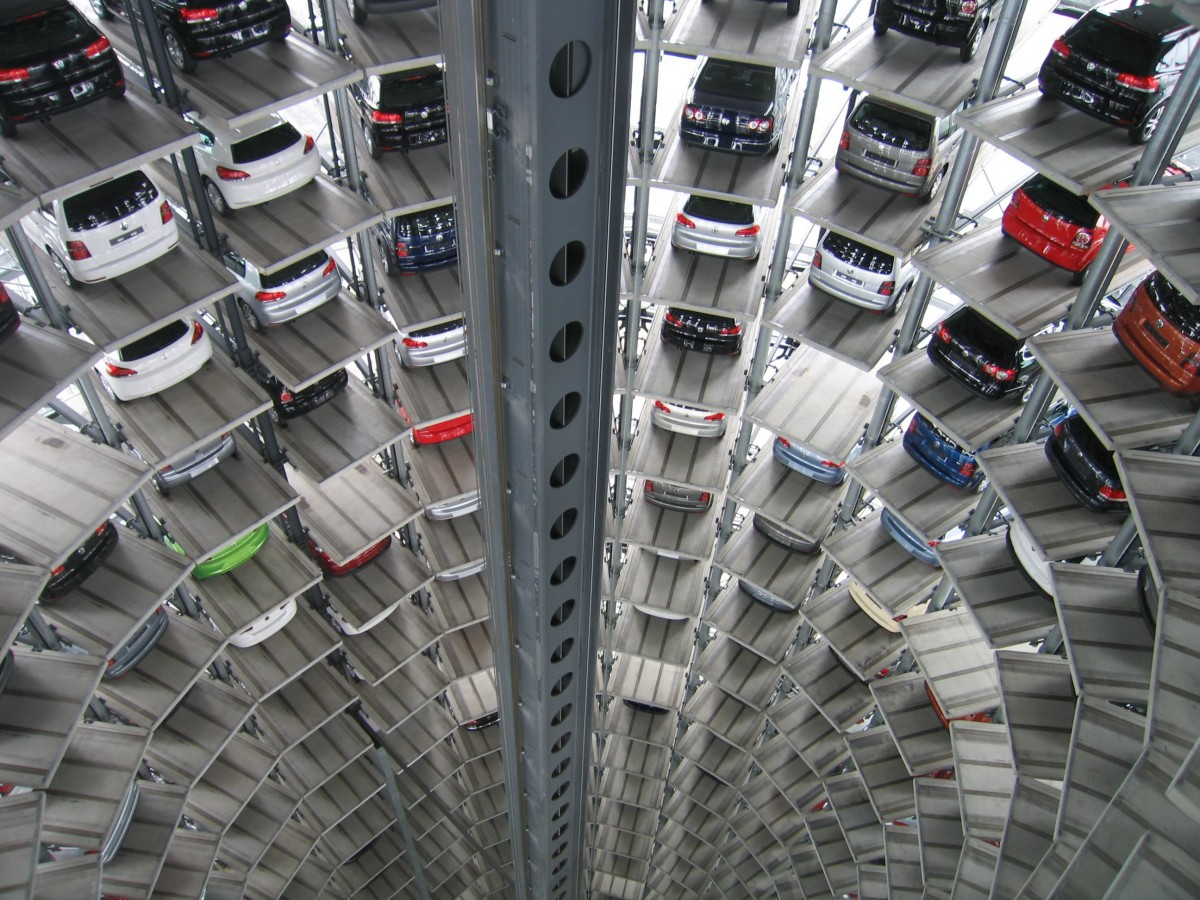
\includegraphics[width=\linewidth]{car-tower}}
	}
\end{frame}
% how to automatically generate products given a descriptive selection of features?

\subsection{Combinatorial Explosion}
\begin{frame}{\insertsubsection}
	\leftorright{
	}{
		\myexampletight{Industrial Configuration Spaces \mysource{\evaluatingsharpsatsolvers}}{
			\centering\evaluatingsharpsatsolverslink{\includegraphics[width=\linewidth,page=6,trim=50 210 320 440,clip]{2020/2020-VaMoS-Sundermann}}
		}
	}
\end{frame}
% huge configuration spaces: Chico's numbers
% expoential grows (in the number of features)
% not all combinations valid
% how to model valid combinations?

\subsection{Feature Interactions}
\begin{frame}{\insertsubsection}
	\leftorright{
		\todots
	}{
		\myexampletight{Invalid Car Configurations}{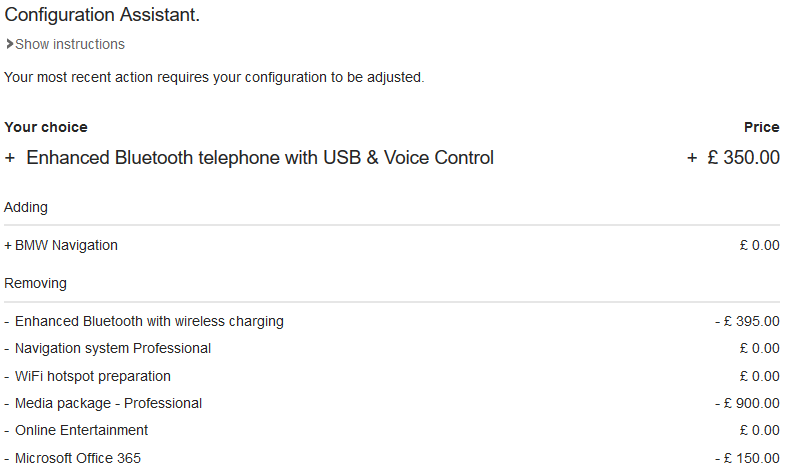
\includegraphics[width=\linewidth]{bmw-series1-confassistant-bluetooth}}
	}
\end{frame}
% typically unknown in advance
% quality assurance/correctness necessary

%\subsection{Incompatible Features}
%% hidden in Ebay, grayed out in Amazon, hints for Lenovo
%\subsection{Compound Features}
%% software for Lenovo, ...
%\subsection{Automated Reconfiguration}
%% BMW, Toyota
%\subsection{Interactive Resolution of Conflicts}
%% Lenovo, Toyota
%\subsection{}

\subsection{Continuous Growth}
\begin{frame}{\insertsubsection}
	\leftorright{
		\todots
	}{
		\todots
	}
\end{frame}
% evolution: number of features/variants increases
% number of features grows over time: picture on linux from ulm slides
% law?

%\subsection{Maintainability}
% maintenance of preprocessor code?

% costs: development, investment, maintenance, logistic, production
% customer needs?

